\documentclass[12pt]{article}
%% arXiv paper template by Flip Tanedo
%% last updated: Dec 2016



%%%%%%%%%%%%%%%%%%%%%%%%%%%%%
%%%  THE USUAL PACKAGES  %%%%
%%%%%%%%%%%%%%%%%%%%%%%%%%%%%

\usepackage{amsmath}
\usepackage{amssymb}
\usepackage{amsfonts}
\usepackage{graphicx}
\usepackage{xcolor}
\usepackage{nopageno}
\usepackage{enumerate}
\usepackage{parskip}


\renewcommand{\thesection}{}
\renewcommand{\thesubsection}{\arabic{subsection}}

%%%%%%%%%%%%%%%%%%%%%%%%%%%%%%%%%%%%%%%%%%%%%%%
%%%  PAGE FORMATTING and (RE)NEW COMMANDS  %%%%
%%%%%%%%%%%%%%%%%%%%%%%%%%%%%%%%%%%%%%%%%%%%%%%

\usepackage[margin=2cm]{geometry}   % reasonable margins

\graphicspath{{figures/}}	        % set directory for figures

% for capitalized things
\newcommand{\acro}[1]{\textsc{\MakeLowercase{#1}}}    

\numberwithin{equation}{section}    % set equation numbering
\renewcommand{\tilde}{\widetilde}   % tilde over characters
\renewcommand{\vec}[1]{\mathbf{#1}} % vectors are boldface

\newcommand{\dbar}{d\mkern-6mu\mathchar'26}    % for d/2pi
\newcommand{\ket}[1]{\left|#1\right\rangle}    % <#1|
\newcommand{\bra}[1]{\left\langle#1\right|}    % |#1>
\newcommand{\Xmark}{\text{\sffamily X}}        % cross out

\let\olditemize\itemize
\renewcommand{\itemize}{
  \olditemize
  \setlength{\itemsep}{1pt}
  \setlength{\parskip}{0pt}
  \setlength{\parsep}{0pt}
}


% Commands for temporary comments
\newcommand{\comment}[2]{\textcolor{red}{[\textbf{#1} #2]}}
\newcommand{\flip}[1]{{\color{red} [\textbf{Flip}: {#1}]}}
\newcommand{\email}[1]{\texttt{\href{mailto:#1}{#1}}}

\newenvironment{institutions}[1][2em]{\begin{list}{}{\setlength\leftmargin{#1}\setlength\rightmargin{#1}}\item[]}{\end{list}}


\usepackage{fancyhdr}		% to put preprint number



% Commands for listings package
%\usepackage{listings}      % \begin{lstlisting}, for code
%
% \lstset{basicstyle=\ttfamily\footnotesize,breaklines=true}
%    sets style to small true-type



%%%%%%%%%%%%%%%%%%%
%%%  HYPERREF  %%%%
%%%%%%%%%%%%%%%%%%%

%% This package has to be at the end; can lead to conflicts
\usepackage{microtype}
\usepackage[
	colorlinks=true,
	citecolor=black,
	linkcolor=black,
	urlcolor=green!50!black,
	hypertexnames=false]{hyperref}





\begin{document}


\begin{center}

    {\Large \textsc{Short HW 2}:
    \textbf{QED}}
    
\end{center}

\vskip .4cm

\noindent
\begin{tabular*}{\textwidth}{rl}
	\textsc{Course:}& Physics 165, \emph{Introduction to Particle Physics} (2022)
	\\
	\textsc{Instructor:}& Prof. Flip Tanedo (\email{flip.tanedo@ucr.edu})
	\\
	\textsc{Due by:}& \textbf{Thursday}, April 7
\end{tabular*}



\section{Quantum Electrodynamics}

The Feynman rules for \textbf{quantum electrodynamics} are:
\begin{center}
	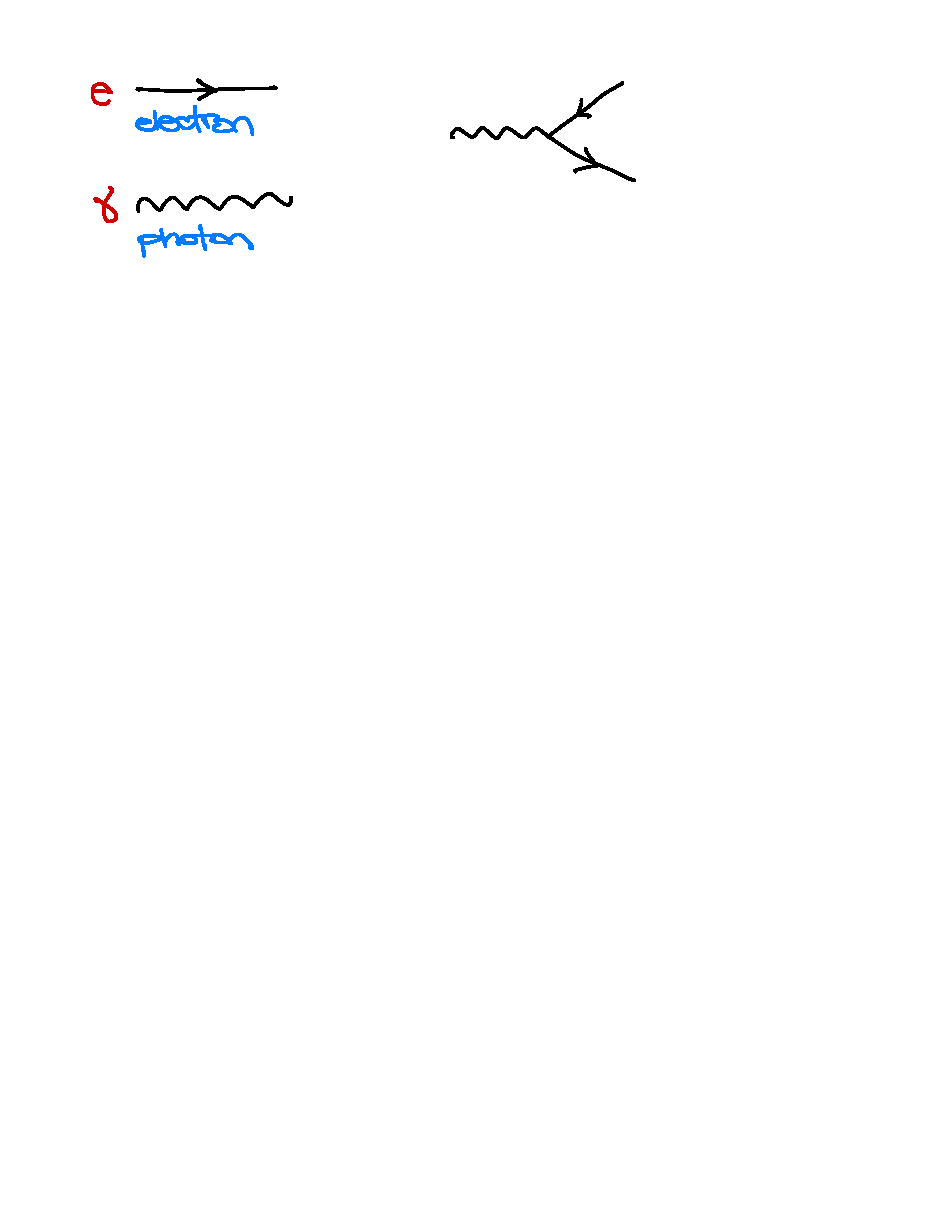
\includegraphics[width=.7\textwidth]{figures/HW2a_QED.pdf}
\end{center}
This corresponds to a theory with two particles: an electron, $e$, and a photon, $\gamma$. The electron has an arrow on it. That indicates that it is distinct from its anti-particle, which we call the \emph{positron}, $\bar e$. You are free to rotate the electron line (``propagator'') so that the arrow points in either direction. If the arrow is flowing with the direction of time (to the right) then the particle is an electron, if the arrow is flowing opposite the direction of time (to the left) then the particle is a positron.

Here's a useful guide for the nomenclature of how to read the in- and out-states of a diagram:
\begin{center}
	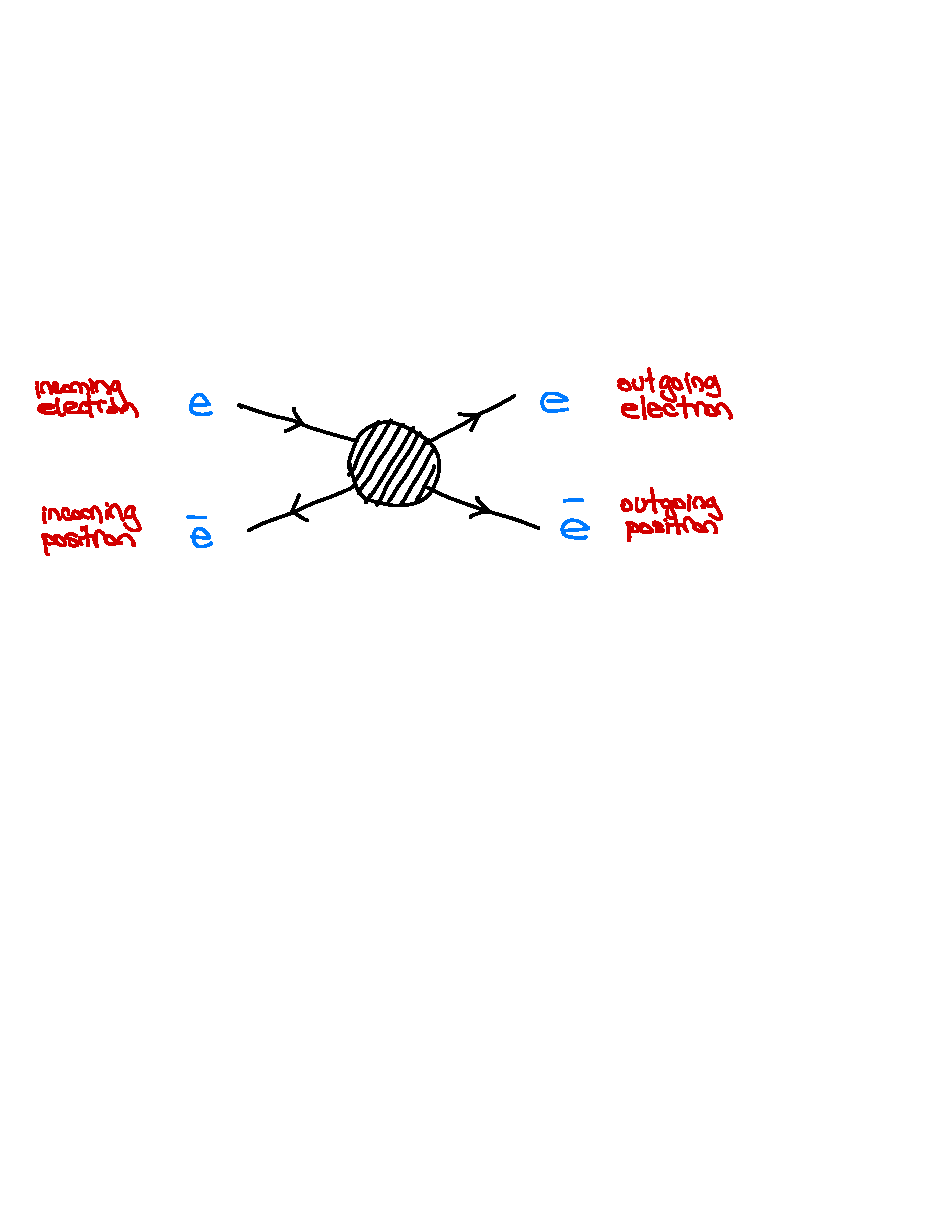
\includegraphics[width=.7\textwidth]{figures/HW2a_nomenclature.pdf}
\end{center}

Reminder of the Feynman Rules game:
\begin{itemize}
	\item You are given a set of \emph{external states}. You have some number of electrons/positrons/photons on the left of the diagram as initial states, and some number of electrons/positrons/photons on the right of the diagram that are the final states. The external states are the only free ends of the diagram, every other line must connect between two vertices.
	\item We would like to draw graphs that connect the initial states to the final states. We restrict to graphs that are totally connected; there must be a path from every piece of the diagram to every other piece.
	\item You may use as many copies of the lines and vertices as you want. You may rotate them, make them curved as needed. Only topology matters. (That also means that it is polite to try to `straighten out' everything once you have a graph.)
	\item Draw diagrams with the fewest number of vertices. But if multiple diagrams have the same number of vertices, you have to include all of them.
	\item If there are multiple diagrams, draw the external states the same for each diagram. That is: fix a convention for the vertical ordering of the external particles, then each diagram is a unique `circuit' between these diagrams.
\end{itemize}

\subsection{Simple processes in QED}

Please draw all of the diagrams at the lowest order\footnote{This means: find a diagram with the fewest number of vertices. Then draw any other topologically distinct diagrams that are at the same order.}, \emph{or} explicitly state that the diagram is not possible. If the diagram is not possible, write a few sentences explaining why based on the Feynman rules. Be careful to note that $e$ is an electron (arrow pointing to the right) and $\bar e$ is a positron (arrow pointing to the left).

\begin{enumerate}[(a)]
\item $e\bar e \to e\bar e$
\item $ee \to ee$
\item $ee \to eee$
\item $e\gamma \to e\gamma$
\item $e \to \gamma \gamma \bar e$
\item $\gamma \gamma \to \gamma \gamma$
\item $e \to e \gamma$
\item $\gamma \to ee\bar e\bar e$
\end{enumerate}
Some of the above diagrams are allowed, but should bother you based on kinematics. Which of these diagrams appear to violate the kinematic conservation laws? (Energy and momentum.)

\end{document}